\chapter*{Introduction}
\addcontentsline{toc}{chapter}{Introduction}
\markboth{Introduction}{Introduction}
\label{chap:introduction}
%\minitoc

\section*{Contexte}
\addcontentsline{toc}{section}{Contexte}

L'entreprise Liebherr est une entreprise familiale allemande fondée en 1949. En 2016, Liebherr employait près de 41000 personnes et son chiffre d'affaire s'élevait à 9 milliard d'euros. Son domaine d'activité est assez varié puisqu'elle fabrique des engins de construction, des machine-outils, des réfrigérateurs ou encore des équipements aéronautiques. Liebherr commercialise notamment des systèmes d'air conditionné qui équipent la totalité des avions de la gamme A320 et assure également leur maintenance.

Liebherr a constaté que plusieurs de ses clients rencontrent parfois les mêmes problèmes de maintenance sur ces systèmes et suppose que ceux-ci sont dû au mode d'utilisation des avions. Afin d'être plus efficace dans sa gestion de la maintenance, Liebherr a souhaité améliorer le suivi des vols des avions contenant leurs systèmes. 

Pour cela, il existe des données open-sources qu'il est possible d'exploiter notamment grâce à l'Automatic Dependent Surveillance-Broadcast (ADS-B). C'est un système de surveillance coopératif pour le contrôle du traffic aérien, qui regroupe la position, vitesse de montée, vitesse de descente et altitude envoyés par les avions à des stations positionnées au sol.

\section*{Objectifs}
\addcontentsline{toc}{section}{Objectifs}

Le but de notre projet est d'établir une classification des compagnies aériennes par modes d'opérations. Ils ont à priori un impact important sur le design des systèmes d'air commercialisés par la société et peuvent expliquer les problèmes rencontrés en service par les compagnies aériennes.

Afin de réaliser cette classification, nous souhaitons exploiter les données de vol ADS-B. Notre objectif principal sera d'établir une classification des compagnies aériennes par modes d'opérations similaires. Cela implique:

\begin{itemize}
	\item extraire des données ADS-B les données de chaque avion de type A320
	\item calculer les phases de vol pour chaque vol
	\item trouver des descripteurs et les calculer pour chaque phase de vol
	\item réaliser une application web pour avoir un aperçu global des données calculées
	\item établir la classification finale à partir des données calculées pour chaque vol
\end{itemize}

\section*{Parties prenantes et Livrables}
\addcontentsline{toc}{section}{Parties prenantes et Livrables}
Notre client est la société Liebherr représentée par Nicolas Canouet qui est chargé de l'encadrement du projet. D'un point de vue gestion de projet, Matthieu Bessac se charge de nous accompagner.

Les livrables demandés sont présentés ci-dessous:
\begin{itemize}
	\item un plan de développement cohérent
	\item un compte-rendu répondant au problème initialement formulé par le client
	\item une soutenance PIE présentant le projet et son déroulement
	\item les codes sources commentés et documentés, afin qu'ils soient facilement utilisable par le client
\end{itemize}



\section*{Contraintes associées au projet}
\addcontentsline{toc}{section}{Contraintes associées au projet}
Notre projet se limite à l'étude des données produites par les avions de la gamme A320 puisque notre client ne cherche qu'à établir une classification pour ce type d'avion.

Pour le reste, la forme des rendus par le client est assez libre. Nous prévoyons donc de présenter nos résultats sous la forme d'une application web accompagnée d'un rapport. Cependant, les personnes impliquées dans le projet ne seront plus disponibles une fois le projet terminé. Nous nous devons donc de faire en sorte que nos rendus soient les plus clairs possible afin que le client puissent exploiter au mieux nos résultats.

La figure \ref{fig:pieuvre} replace le projet dans son contexte à l'aide d'un diagramme pieuvre.

\begin{figure}[!ht]
	\centering
	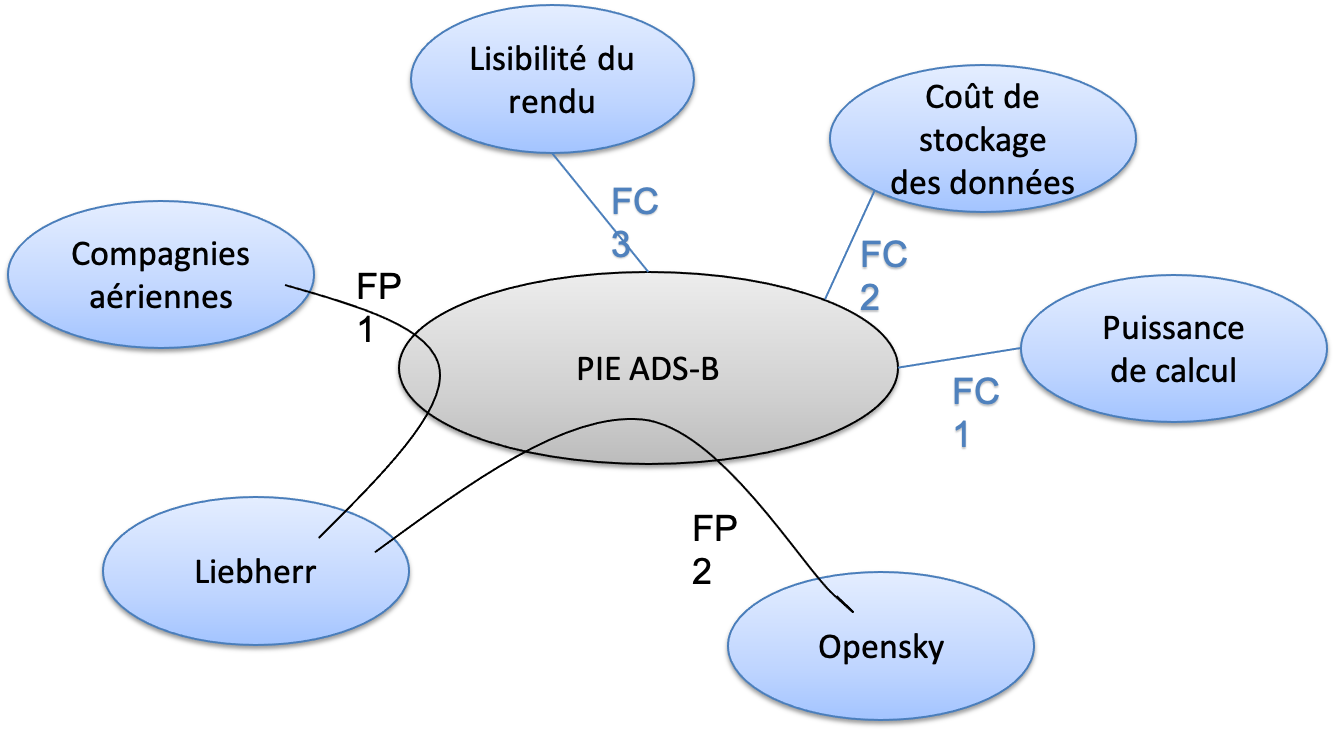
\includegraphics[width=15cm]{DiagrammePieuvre}
	\caption{
		Diagramme pieuvre du projet. FP1: classer les compagnies
		en fonction de leurs modes d'opération, FP2: exploiter les données ADS-B, 
		FC1: ne pas dépasser les ressources informatiques disponibles,
		FC2: respecter les coûts associés au stockage des données,
		FC3: rendre un projet exploitable par le client.
	}
	\label{fig:pieuvre}
\end{figure}


%%% Local Variables: 
%%% mode: latex
%%% TeX-master: "isae-report-template"
%%% End: 
